A continuaci\'on se muestra el diagram en bloques del Hardware y los delimitadores de las secciones, siendo estas:
\begin{itemize}
\item Potencia
\item Cargador
\item Sensado
\end{itemize}

\begin{figure}[H]
	\centering
	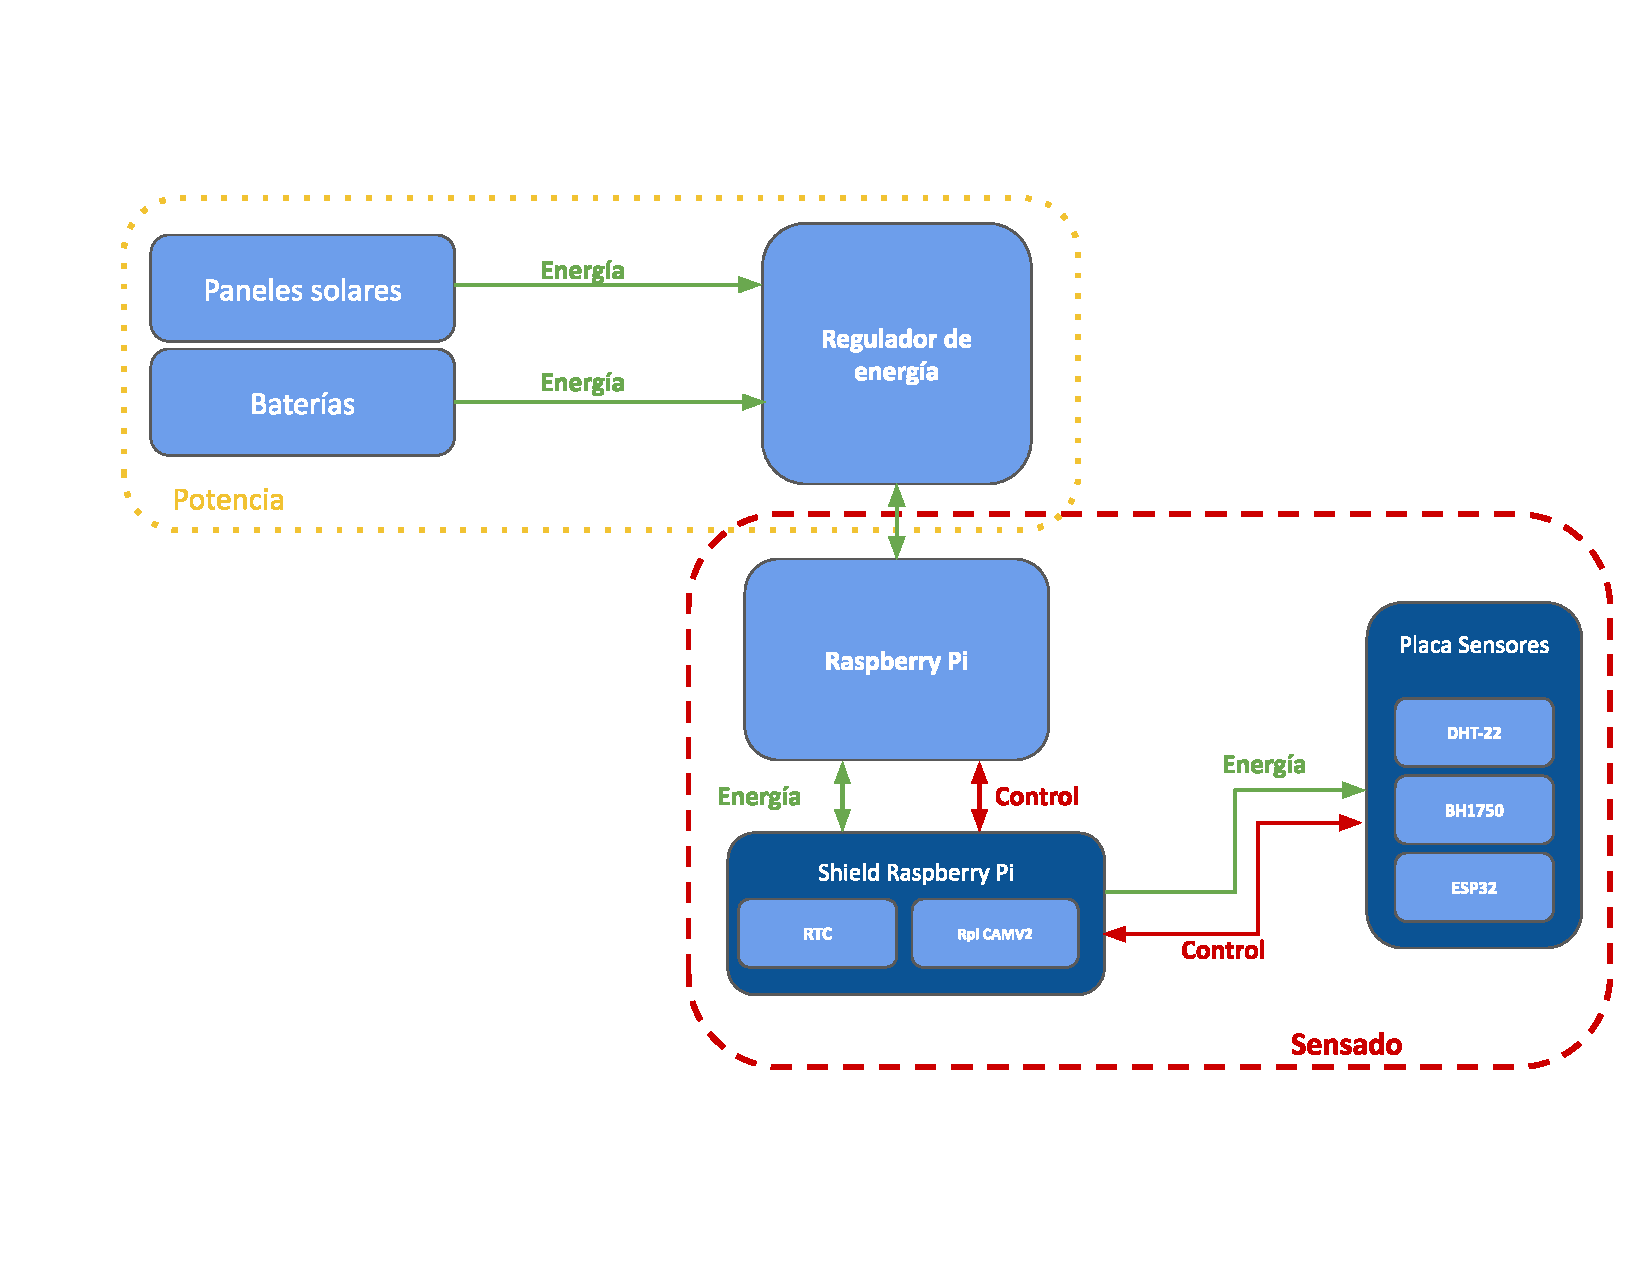
\includegraphics[width=0.7\linewidth]{ImagenesIngenieria de Detalle/DiagramaHardwareMarcado}
	\label{fig:diagrama_hardware}
	\caption{Diagrama en bloques del sistema de hardware.}
\end{figure}
La etapa de potencia es el conjunto de elementos necesarios para proveer de energ\'ia a toda la electr\'onica del proyecto.

El cargador es la etapa que se encarga, como su nombre indica realizar al carga inal\'ambrica de la UBM.

Y la de sensado se encarga de la medici\'on de las variables f\'isicas y de su correcto almacenamiento, teniendo en cuenta que esto implica un conocimiento preciso de la hora.

